%!TEX root = main.tex
%%% Polynomials
\part{}

\section{Quadratics \& Their Applications}

\begin{ques}
What is a quadratic's graph?
\end{ques}

\ifprintanswers
\else
\begin{center}

\begin{tikzpicture}[scale=0.4]
\draw[step=1cm,gray,very thin] (-7,-7) grid (7,7);
\draw (-7,0) -- (7,0);
\draw (0,-7) -- (0,7);
\end{tikzpicture}
\hspace{1in}

\begin{tikzpicture}[scale=0.4]
\draw[step=1cm,gray,very thin] (-7,-7) grid (7,7);
\draw (-7,0) -- (7,0);
\draw (0,-7) -- (0,7);
\end{tikzpicture}
\end{center}
\fi

We call these shapes \blank{parabolas}{parabolas}.

\subsection{Standard form}

\begin{definition}\label{def: std form parabola}
The following is the \emph{standard form} of a parabola with \emph{vertex} $(h,k)$:
\[
f(x)=\blank{a(x-h)^2+k}{a(x-h)^2+k}
\]
If $\blank{a>0}{a>0}$ then the quadratic opens up,
and if $\blank{a<0}{a<0}$ then the quadratic opens
down. We call $\blank{x=h}{x=h}$ the \emph{axis of symmetry}.
\end{definition}

\subsubsection*{Basic quadratic}

\ifprintanswers
\else
\begin{center}
\raisebox{-6em}{
\begin{tikzpicture}[scale=0.4]
\draw[step=1cm,gray,very thin] (-7,-7) grid (7,7);
\draw (-7,0) -- (7,0);
\draw (0,-7) -- (0,7);
\end{tikzpicture}}
\hspace{1in}
\begin{tabular}{rl}
Vertex: & $\blank{(0,0)}{(0,0)}$\\
Axis of Symmetry: & $\blank{x=0}{x=0}$\\
Scale: & $\blank{a=1}{a=1}$
\end{tabular}
\end{center}
\fi

\ifprintanswers\else\newpage\fi

\begin{exercise}
Graph $f(x)=(x-2)^2+1$ below.
\end{exercise}

\ifprintanswers
\else
\begin{center}

\begin{tikzpicture}[scale=0.4]
\draw[step=1cm,gray,very thin] (-7,-7) grid (7,7);
\draw (-7,0) -- (7,0);
\draw (0,-7) -- (0,7);
\end{tikzpicture}
\end{center}
\fi

\vspace{0.5em}

\begin{exercise}
Graph $f(x)=-2(x-1)^2+2$ below.
\end{exercise}

\ifprintanswers
\else
\begin{center}

\begin{tikzpicture}[scale=0.4]
\draw[step=1cm,gray,very thin] (-7,-7) grid (7,7);
\draw (-7,0) -- (7,0);
\draw (0,-7) -- (0,7);
\end{tikzpicture}
\end{center}
\fi

\vspace{0.5em}

\subsection{General form}

\begin{definition}\label{def: gen form quadratic}
The \emph{general form} of a quadratic is as follows:
\[
f(x)=\blank{ax^2+bx+c}{ax^2+bx+c}
\]
\begin{itemize}
\item Vertex: $\blank{\left(\frac{-b}{2a},f\left(\frac{-b}{2a}\right)\right)}{\left(\frac{-b}{2a},f\left(\frac{-b}{2a}\right)\right)}$
\item Axis of Symmetry: $\blank{x=\frac{-b}{2a}}{x=\frac{-b}{2a}}$.
\end{itemize}
\end{definition}

So standard form is good for graphing, but we tend to see most quadratics in general form.
As such, we will need to be able to change between the two forms.

\ifprintanswers\else\newpage\fi

\begin{exercise}
What is the standard form of
\[
f(x)=x^2-4x+2
\]
\end{exercise}
\begin{solution}[3.5in]

\end{solution}

\vspace{0.5em}

\begin{exercise}
Write $f(x)=2x^2+12x+3$ in standard form.
\end{exercise}
\begin{solution}[4in]

\end{solution}

\vspace{0.5em}

\subsection{Determining the equation from the graph}

\begin{exercise}
Find the equation of the following parabola in both standard and general form:
\begin{center}
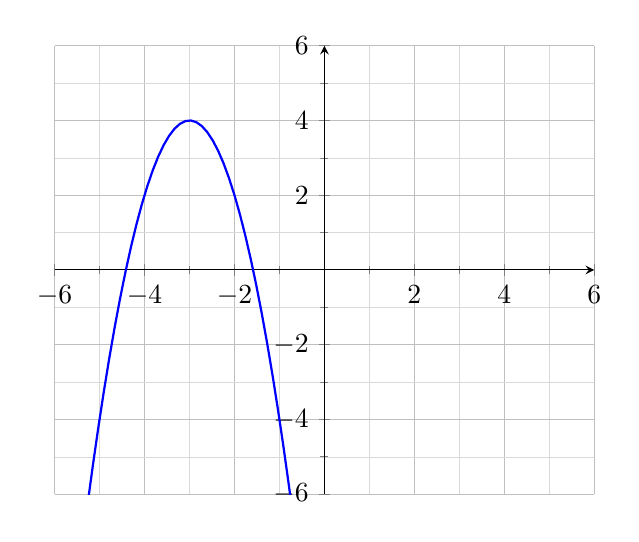
\begin{tikzpicture}
     \begin{axis}%
    [grid=both,
    ymin=-6, ymax=6,
    xmin=-6, xmax=6,
     minor tick num=1,
     grid style={line width=.1pt, draw=gray!30},
     major grid style={line width=.2pt,draw=gray!50},
     axis lines=middle,
     enlargelimits=false,
     domain=-6:6,
     samples=100
    ]
    \addplot+[blue,mark=none,thick] {-2*x^2 -12*x-14};
  \end{axis}
\end{tikzpicture}
\end{center}
\end{exercise}
\begin{solution}[3.5in]

\end{solution}

\ifprintanswers\else\newpage\fi

\begin{exercise}
Find both the standard and general form of $f(x)$ below:
\begin{center}
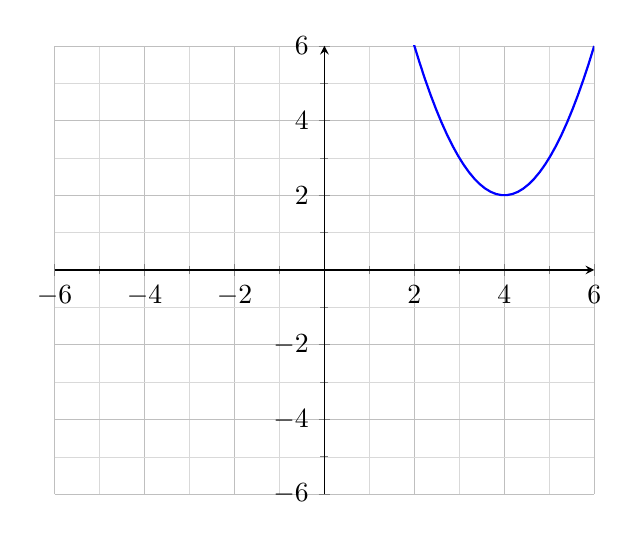
\begin{tikzpicture}
     \begin{axis}%
    [grid=both,
    ymin=-6, ymax=6,
    xmin=-6, xmax=6,
     minor tick num=1,
     grid style={line width=.1pt, draw=gray!30},
     major grid style={line width=.2pt,draw=gray!50},
     axis lines=middle,
     enlargelimits=false,
     domain=-6:6,
     samples=100
    ]
    \addplot+[blue,mark=none,thick] {x^2 -8*x+18};
  \end{axis}
\end{tikzpicture}
\end{center}
\end{exercise}
\begin{solution}[3.5in]

\end{solution}

\ifprintanswers\else\newpage\fi

\subsection{Using intercepts to find the equation}

Sometimes the vertex is not a nice point that we can see, but the intercepts
are nice such as the following problem:

\vspace{0.5em}

\begin{exercise}
Find the general form of $f(x)$ below:
\begin{center}
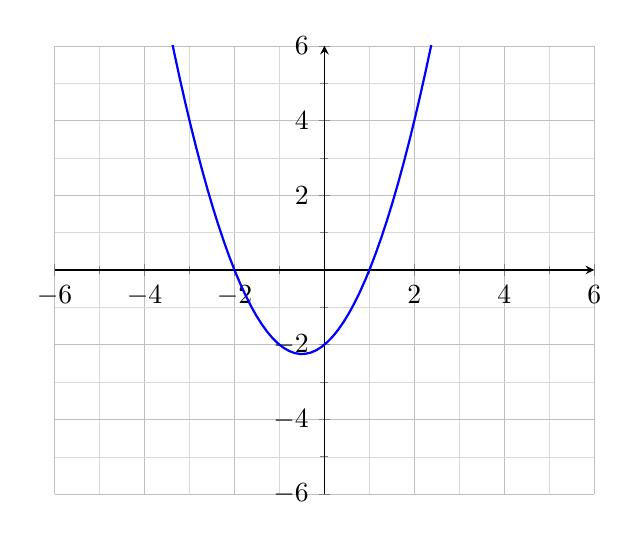
\begin{tikzpicture}
     \begin{axis}%
    [grid=both,
    ymin=-6, ymax=6,
    xmin=-6, xmax=6,
     minor tick num=1,
     grid style={line width=.1pt, draw=gray!30},
     major grid style={line width=.2pt,draw=gray!50},
     axis lines=middle,
     enlargelimits=false,
     domain=-6:6,
     samples=100
    ]
    \addplot+[blue,mark=none,thick] {x^2+x-2};
  \end{axis}
\end{tikzpicture}
\end{center}
\end{exercise}
\begin{solution}[3.5in]

\end{solution}

\subsection{Finding domain \& range from equations}

\ifprintanswers
\else
\begin{center}
\raisebox{-6em}{
\begin{tikzpicture}[scale=0.4]
\draw[step=1cm,gray,very thin] (-7,-7) grid (7,7);
\draw (-7,0) -- (7,0);
\draw (0,-7) -- (0,7);
\end{tikzpicture}}
\hspace{1in}
\begin{tabular}{rl}
Domain: & $\blank{(-\infty,\infty)}{(-\infty\infty)}$\\
(if $a>0$) Range: & $\blank{[k,\infty)}{[k,\infty)}$\\
(if $a<0$) Range: & $\blank{(-\infty,k]}{(-\infty,k]}$
\end{tabular}
\end{center}
\fi

\begin{exercise}
Find the domain and range of $f(x)=(x+3)^2-4$
\end{exercise}
\begin{solution}[2in]

\end{solution}

\vspace{0.5em}

\begin{exercise}
Find the domain and range of $f(x)=-3x^2+12x+17$
\end{exercise}
\begin{solution}[3.5in]

\end{solution}

\subsection{Finding intercepts from the equation}

\begin{exercise}
Find the $x$- and $y$-intercepts of $f(x)=2x^2-4x-6$.
\end{exercise}
\begin{solution}[3in]

\end{solution}

\subsection{Maximum and Minimum values of quadratics}

\begin{note}
The max/min value always occur at the \blank{$y$ value of the vertex}{$y$ value of the vertex}.
\begin{itemize}
    \item If $a>0$ it has a \blank{minimum value}{minimum value},
    \item and if $a<0$ it has a \blank{maximum value}{maximum value}.
\end{itemize}
\end{note}

\begin{exercise}
A farmer is building a fence to enclose a rectangular area next to a wall.
They have 164 ft of fence to use. What is the largest area they can enclose in fence?
\end{exercise}
\begin{solution}[3in]

\end{solution}

\begin{exercise}
Find the dimensions with the maximum area that is fenced in using the shape below and using 234 ft of fence.
\begin{center}
\begin{tikzpicture}
\draw (0,0) -- (6,0) -- (6,3) -- (0,3) -- cycle;
\draw (3,0) -- (3,3);
\end{tikzpicture}  
\end{center}

\end{exercise}
\begin{solution}[2in]

\end{solution}

\section{Polynomials}

\begin{definition}\label{def: power function}
A \emph{power function} is a function that can be written as
\[
f(x)=\blank{kx^n}{kx^n}
\]
\end{definition}
\begin{example}
\text{}
\begin{itemize}
    \item $\blank{f(x)=3x^2}{f(x)=3x^2}$
    \item $\blank{f(x)=7\sqrt[3]{x}=7x^{1/3}}{f(x)=7\sqrt[3]{x}=7x^{1/3}}$
\end{itemize}
\end{example}

\begin{nonex}
\text{}
\begin{itemize}
    \item $\blank{f(x)=5\cdot3^x}{f(x)=5\cdot3^x}$
    \item $\blank{f(x)=2x^2+7x}{f(x)=2x^2+7x}$
\end{itemize}
\end{nonex}

Having defined polynomials before (see Definition \ref{def: polynomial}), we can define them sightly differently using power functions as follows:

\begin{definition}\label{def: polynomial 2}
A \emph{polynomial} is a sum of power functions such that all of the powers are natural numbers (non-negative integers) with the following 
form:
\[
f(x)=a_nx^n+a_{n-1}x^{n-1}+\cdots+a_1x+a_0.
\]
\end{definition}

Recall that $a_n$ is called the leading coefficient, $a_nx^n$
is the leading term and $n$ is the degree of $f(x)$.

\vspace{0.5em}

\begin{example}
\text{}
\begin{itemize}
    \item $\blank{f(x)=3x^2}{f(x)=3x^2}$
    \item $\blank{f(x)=2x^2+7x}{f(x)=2x^2+7x}$
    \item $\blank{f(x)=5x^7+3x^2-4}{f(x)=5x^7+3x^2-4}$
\end{itemize}
\end{example}

\vspace{0.5em}

\begin{nonex}
\text{}
\begin{itemize}
    \item $\blank{f(x)=3x^2+7x^{1/2}}{f(x)=3x^2+7x^{1/2}}$
\end{itemize}
\end{nonex}

\subsection{Graphs of Polynomials}

The graphs of polynomials have 3 key properties:
\begin{enumerate}[1)]
    \item \blank{smooth}{smooth} - the graph has no sharp corners.
    \item \blank{continuous}{continuous} - no jumps or breaks in the graph.
    \item \blank{No Asymptotes}{No Asymptotes}
\end{enumerate}

\begin{ques}
What is an \blank{asymptote}{asymptote}?
\end{ques}

\begin{itemize}
    \item \blank{Vertical Asymptotes (VA)}{Vertical Asymptotes (VA)} - 
    vertical lines that a function approaches by cannot cross.
    \item \blank{Horizontal Asymptotes (HA)}{Horizontal Asymptotes (HA)} - horizontal lines that a function approaches as $x\rightarrow\infty$ or $x\rightarrow-\infty$.
\end{itemize}

\ifprintanswers\else\newpage\fi

Here are some visualizations of these different properties:

\vspace{2em}

\ifprintanswers
\else
\begin{center}

\begin{tikzpicture}[scale=0.5]
\draw[step=1cm,gray,very thin] (-5,-5) grid (5,5);
\draw (-5,0) -- (5,0);
\draw (0,-5) -- (0,5);
\end{tikzpicture}
\hspace{1in}

\begin{tikzpicture}[scale=0.5]
\draw[step=1cm,gray,very thin] (-5,-5) grid (5,5);
\draw (-5,0) -- (5,0);
\draw (0,-5) -- (0,5);
\end{tikzpicture}
\end{center}
\vspace{1em}
\begin{center}

\begin{tikzpicture}[scale=0.5]
\draw[step=1cm,gray,very thin] (-5,-5) grid (5,5);
\draw (-5,0) -- (5,0);
\draw (0,-5) -- (0,5);
\end{tikzpicture}
\hspace{1in}

\begin{tikzpicture}[scale=0.5]
\draw[step=1cm,gray,very thin] (-5,-5) grid (5,5);
\draw (-5,0) -- (5,0);
\draw (0,-5) -- (0,5);
\end{tikzpicture}
\end{center}
\fi

\ifprintanswers\else\newpage\fi

\begin{exercise}
Which of the following are polynomials?
\begin{center}
\raisebox{10em}{(A) }
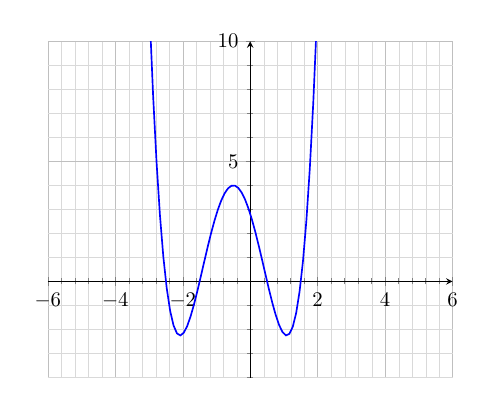
\begin{tikzpicture}[scale=0.75]
     \begin{axis}%
    [grid=both,
     minor tick num=4,
     ymin=-4, ymax=10,
     xmin=-6, xmax=6,
     grid style={line width=.1pt, draw=gray!30},
     major grid style={line width=.2pt,draw=gray!50},
     axis lines=middle,
     enlargelimits=false,
     samples=100
    ]
    \addplot+[blue,mark=none,thick] {(x-0.5)*(x+1.5)*(x-1.5)*(x+2.5)};
  \end{axis}
\end{tikzpicture}
\hspace{1in}
\raisebox{10em}{(B) }
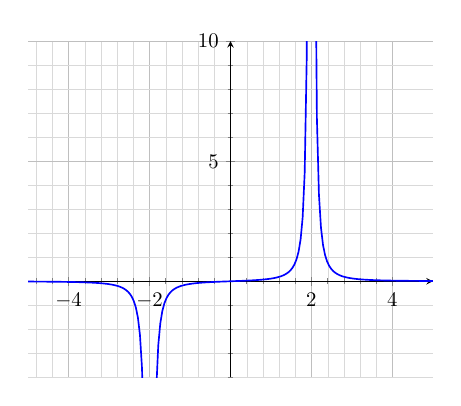
\begin{tikzpicture}[scale=0.75]
     \begin{axis}%
    [grid=both,
     minor tick num=4,
     ymin=-4, ymax=10,
     grid style={line width=.1pt, draw=gray!30},
     major grid style={line width=.2pt,draw=gray!50},
     axis lines=middle,
     enlargelimits=false,
     samples=200
    ]
    \addplot+[blue,mark=none,thick] {x/((x+2)*(x+2)*(x-2)*(x-2))};
  \end{axis}
\end{tikzpicture}
\end{center}
\vspace{1em}
\begin{center}
\raisebox{10em}{(C) }
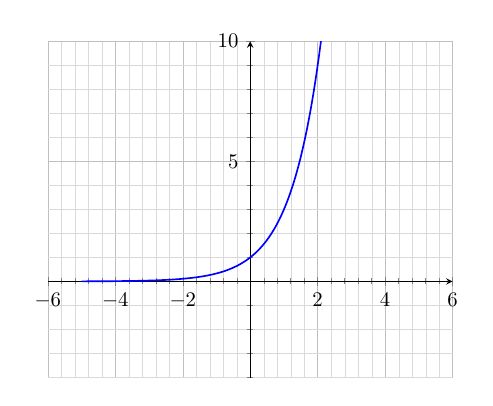
\begin{tikzpicture}[scale=0.75]
     \begin{axis}%
    [grid=both,
     minor tick num=4,
     ymin=-4, ymax=10,
     xmin=-6, xmax=6,
     grid style={line width=.1pt, draw=gray!30},
     major grid style={line width=.2pt,draw=gray!50},
     axis lines=middle,
     enlargelimits=false,
     samples=200
    ]
    \addplot+[blue,mark=none,thick] {3^x};
  \end{axis}
\end{tikzpicture}
\hspace{1in}
\raisebox{10em}{(D) }
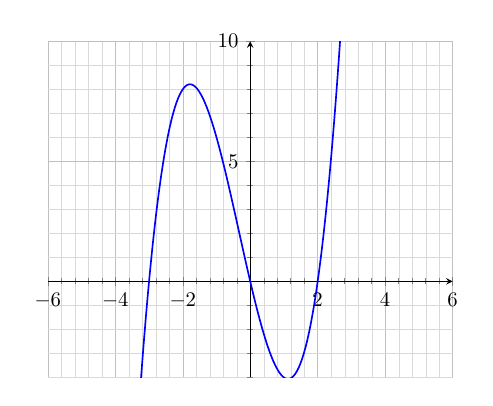
\begin{tikzpicture}[scale=0.75]
     \begin{axis}%
    [grid=both,
     minor tick num=4,
     ymin=-4, ymax=10,
     xmin=-6, xmax=6,
     grid style={line width=.1pt, draw=gray!30},
     major grid style={line width=.2pt,draw=gray!50},
     axis lines=middle,
     enlargelimits=false,
     samples=200
    ]
    \addplot+[blue,mark=none,thick] {x*(x-2)*(x+3)};
  \end{axis}
\end{tikzpicture}
\end{center}
\end{exercise}

\subsection{End behavior of a polynomial}

The end behavior of a polynomial describes what $f(x)$ is 
doing as $x\rightarrow\blank{\infty}{\infty}$ or\\ $x\rightarrow\blank{-\infty}{-\infty}$.

\vspace{0.5em}

\begin{ques}
What do we need from a polynomial's equation to determine the end behavior?
\end{ques}

\vspace{0.5em}

\begin{prop}
If $f(x)=a_nx^n+a_{n-1}^{n-1}+\cdots$, then the end behavior of $f(x)$ can be
categorized as follows:
\begin{center}
\begin{tabular}{c|c|c}
 & $n$ even  & $n$ odd \\\hline
$a_n>0$ & \phantom{$\dl==\Bigg(\frac{A}{B}==$} & \phantom{$\dl===\Bigg(\frac{A}{B}==$}  \\\hline
$a_n<0$ & \phantom{$\dl===\Bigg(\frac{A}{B}==$}  & \phantom{$\dl===\Bigg(\frac{A}{B}==$} 
\end{tabular}
or
\begin{tabular}{c|c|c}
 & $n$ even  & $n$ odd \\\hline
$a_n>0$ & \phantom{$\dl===\Bigg(\frac{A}{B}==$} & \phantom{$\dl===\Bigg(\frac{A}{B}==$}  \\\hline
$a_n<0$ & \phantom{$\dl===\Bigg(\frac{A}{B}==$}  & \phantom{$\dl===\Bigg(\frac{A}{B}==$} 
\end{tabular}
\end{center}
\end{prop}

\ifprintanswers\else\newpage\fi

\begin{exercise}
What is the end behavior of $f(x)=18x^3+2$
\end{exercise}
\begin{solution}[1in]

\end{solution}

\vspace{0.5em}

\begin{exercise}
Describe the end behavior of
\[
f(x)=-5x(x-4)(x+5)(2x+3)
\]
\end{exercise}
\begin{solution}[1in]

\end{solution}

\vspace{0.5em}

\begin{exercise}
Which of the following factors would cause the graph of $f(x)$ to decrease
as $x$ goes to negative infinity?
\[
f(x)=(2x^2+5)(x-7)
\]
\end{exercise}
\begin{checkboxes}
\choice $-3$
\CorrectChoice $5x^2$
\choice $4(2x-7)$
\end{checkboxes}
\begin{solution}[3in]

\end{solution}

\subsection{Identifying intercepts}

Recall that $x$-intercepts are where $\blank{f(x)=0}{f(x)=0}$, and the
$y$-intercept is at $\blank{f(0)}{f(0)}$.

\begin{exercise}
What are the intercepts of
\[
f(x)=(x-5)(x+3)(x-1)
\]
\end{exercise}

\begin{solution}[2in]

\end{solution}

\subsection{Finding zeros}

There are two steps to finding the zeros of a polynomial:
\begin{enumerate}[1)]
    \item \blank{Factor out the GCF (if there is one)}{Factor out the GCF (if there is one)}
    \item \blank{Factor the remaining polynomial}{Factor the remaining polynomial}
\end{enumerate}

\vspace{0.5em}

\begin{exercise}
Find the zeros of $f(x)=x^5-14x^4+49x^3$
\end{exercise}
\begin{solution}[3in]

\end{solution}

\subsection{More on graphs and degrees}

\begin{definition}\label{def: turning point}
A \emph{turning point} is a point where $f(x)$
changes from \blank{increasing to}{increasing to} \blank{decreasing or vice-versa}{decreasing or vice-versa}.
\end{definition}

\begin{center}

\begin{tikzpicture}[scale=0.75]
\draw[step=1cm,gray,very thin] (-5,-5) grid (5,5);
\draw (-5,0) -- (5,0);
\draw (0,-5) -- (0,5);
\end{tikzpicture}
\end{center}

Here are two facts relating to the degree of a polynomial and its graph.

 \begin{fact}
A polynomial of degree $n$ can have at most $\blank{n-1}{n-1}$ turning points.
\end{fact}

\begin{fact}
A polynomial of degree $n$ can have at most $\blank{n}{n}$ $x$-intercepts.
\end{fact}

\begin{exercise}
If a polynomial has $7$ $x$-intercepts, what can you say about the degree?
\end{exercise}
\begin{solution}[1in]

\end{solution}

\begin{exercise}
If the degree of a polynomial is $8$, what can you say about the number of turning points?
\end{exercise}
\begin{solution}[1in]

\end{solution}

\subsection{More about zeros}

What follows is one of the most important theorems in algebra, but we need one definition first.

\begin{definition}
If $b$ is a zero of a polynomial $f(x)$, then the \emph{multiplicity} of $b$ is the number of times that $b$ appears as a zero to $f(x)$.
\end{definition}

\begin{theorem}[Fundamental Theorem of Algebra]\label{thm: FTA}
If we allow complex numbers, then any polynomial can be completely factored into linear
factors of its zeros. That is if $f(x)$ is a polynomial and $b_1,b_2,\ldots,b_k$ are the
zeros of $f(x)$ with multiplicities $m_1,m_2,\ldots,m_k$, we can write $f(x)$ as follows:
\[
f(x)=a(x-b_1)^{m_1}(x-b_2)^{m_2}\cdots(x-b_k)^{m_k}
\]
\end{theorem}

\begin{example}
The polynomial $f(x)=(x-3)^2(x+4)^6$ has zeros at $\blank{x=3}{x=3}$ and
$\blank{x=-4}{x=-4}$ with multiplicities $\blank{2}{2}$ and $\blank{6}{6}$, respectively.
\end{example}

\begin{note}
A consequence of the Fundamental Theorem of Algebra is
\[
m_1+m_2+\cdots+m_k=\blank{\deg(f)}{\deg(f)}
\]
\end{note}

The multiplicities have an effect on how the graph acts around the corresponding
zero ($x$-intercept).

\begin{itemize}
    \item If the multiplicity of the zero $b$ is odd, then 
\begin{center}
\rule{1in}{0.1pt}\quad\text{or}\quad\rule{1in}{0.1pt}
\end{center}
\item If the multiplicity of the zero $b$ is even, then 
\begin{center}
\rule{1in}{0.1pt}\quad\text{or}\quad\rule{1in}{0.1pt}
\end{center}
\end{itemize}

\vspace{0.5em}

Additionally, the flatter the graph is around the zero the larger the multiplicity.

\vspace{0.5em}

Using these ideas we can make conclusions about the multiplicity of zeros based
on the graph of a polynomial and some information about the degree.

\ifprintanswers\else\newpage\fi

\begin{exercise}
Given that $f(x)$ below is a degree 4 polynomial, find
the zeros and their multiplicities:
\begin{center}
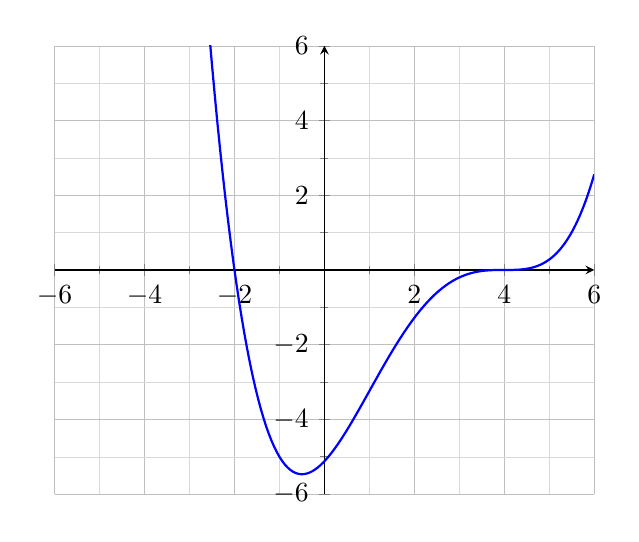
\begin{tikzpicture}
\begin{axis}%
    [grid=both,
     minor tick num=1,
     ymin=-6, ymax=6,
     xmin=-6, xmax=6,
     grid style={line width=.1pt, draw=gray!30},
     major grid style={line width=.2pt,draw=gray!50},
     axis lines=middle,
     enlargelimits=false,
     domain=-6:6,
     samples=200
    ]
    \addplot+[blue,mark=none,thick] {1/25*(x-4)^3*(x+2)};
  \end{axis}
\end{tikzpicture}
\end{center}
\end{exercise}
\begin{solution}[3in]

\end{solution}

\subsection{The Intermediate Value Theorem}

\begin{center}

\begin{tikzpicture}[scale=0.75]
\draw[step=1cm,gray,very thin] (-2,-4) grid (8,4);
\draw (-2,0) -- (8,0);
\draw (0,-4) -- (0,4);
\end{tikzpicture}
\end{center}

\begin{theorem}[Intermediate Value Theorem]\label{thm: IVT}
For a continuous function (think polynomial) $f(x)$ on $[a,b]$
and a number $z$ in between $f(a)$ and $f(b)$, there exists a $c$
in $[a,b]$ such that $f(c)=z$.
\end{theorem}

\begin{ques}
Do we care?
\end{ques}

This theorem is useful for \blank{``finding zeros''}{``finding zeros''} because
if $\blank{0}{0}$ is between $f(a)$ and $f(b)$ and $f$ is continuous on $[a,b]$,
then the IVT says that there is a $c$ in $[a,b]$ such that $f(c)=\blank{0}{0}$.


\begin{note}
$\blank{0}{0}$ is between $f(a)$ and $f(b)$ $\Longleftrightarrow$
$f(a)$ and $f(b)$ \blank{have different signs}{have different signs}
\end{note}

\begin{center}

\begin{tikzpicture}[scale=0.5]
\draw[step=1cm,gray,very thin] (-2,-3) grid (8,3);
\draw (-2,0) -- (8,0);
\draw (0,-3) -- (0,3);
\end{tikzpicture}
\end{center}

\begin{exercise}
Show that $f(x)=3x^2-1$ has a zero in $[-1,0]$ using IVT.
\end{exercise}
\begin{solution}[2in]

\end{solution}

\begin{exercise}
Does IVT guarantee that $f(x)=x^2-4x+4$ have a zero between $[1,4]$? 
\end{exercise}
\begin{solution}[2in]

\end{solution}

\subsection{Drawing conclusions from graphs of polynomials}

\begin{exercise}
Describe the leading coefficient and degree of the following polynomial:
\begin{center}
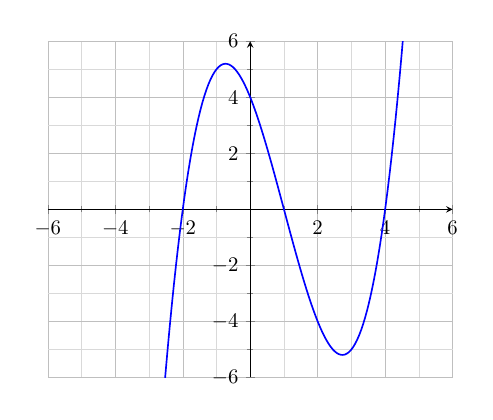
\begin{tikzpicture}[scale=0.75]
\begin{axis}%
    [grid=both,
     minor tick num=1,
     ymin=-6, ymax=6,
     xmin=-6, xmax=6,
     grid style={line width=.1pt, draw=gray!30},
     major grid style={line width=.2pt,draw=gray!50},
     axis lines=middle,
     enlargelimits=false,
     domain=-6:6,
     samples=200
    ]
    \addplot+[blue,mark=none,thick] {1/2*(x-4)*(x+2)*(x-1)};
  \end{axis}
\end{tikzpicture}
\end{center}
\end{exercise}
\begin{solution}[1in]

\end{solution}
\begin{exercise}
Describe the leading coefficient and degree of the following polynomial:
\begin{center}
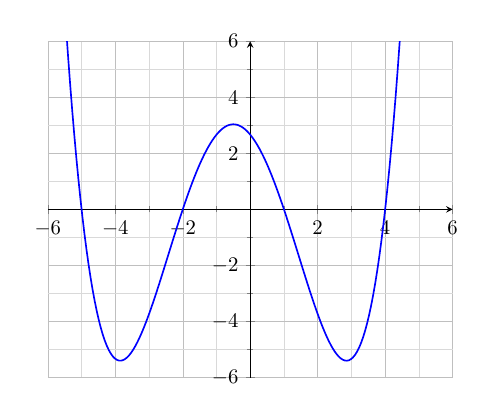
\begin{tikzpicture}[scale=0.75]
\begin{axis}%
    [grid=both,
     minor tick num=1,
     ymin=-6, ymax=6,
     xmin=-6, xmax=6,
     grid style={line width=.1pt, draw=gray!30},
     major grid style={line width=.2pt,draw=gray!50},
     axis lines=middle,
     enlargelimits=false,
     domain=-6:6,
     samples=200
    ]
    \addplot+[blue,mark=none,thick] {1/15*(x-4)*(x+5)*(x+2)*(x-1)};
  \end{axis}
\end{tikzpicture}
\end{center}
\end{exercise}
\begin{solution}[1in]

\end{solution}

\ifprintanswers\else\newpage\fi

\subsection{Graphing Polynomials}

\begin{exercise}
Graph $f(x)=4(x-2)(x+1)(x+6)$.
\end{exercise}
\ifprintanswers
\else
\begin{center}

\begin{tikzpicture}[scale=0.5]
\draw[step=1cm,gray,very thin] (-8,-8) grid (8,8);
\draw (-8,0) -- (8,0);
\draw (0,-8) -- (0,8);
\end{tikzpicture}
\hspace{3in}\phantom{=}
\end{center}
\fi

\begin{exercise}
Graph $f(x)=-2(x-6)(x-2)(x+3)$.
\end{exercise}
\ifprintanswers
\else
\begin{center}

\begin{tikzpicture}[scale=0.5]
\draw[step=1cm,gray,very thin] (-8,-8) grid (8,8);
\draw (-8,0) -- (8,0);
\draw (0,-8) -- (0,8);
\end{tikzpicture}
\hspace{3in}\phantom{=}
\end{center}
\fi

\ifprintanswers\else\newpage\fi

\subsection{Finding the equation from the graph}

\begin{exercise}
The graph of the polynomial $f(x)$ is given below. If $f(x)$
is degree 3, find the equation of $f(x)$
\begin{center}
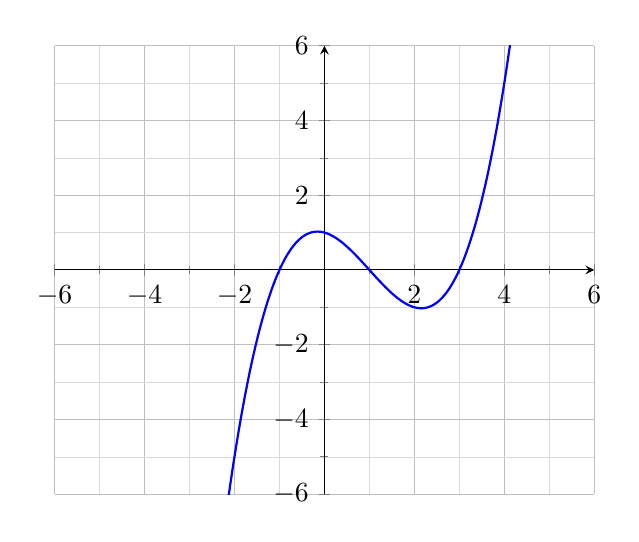
\begin{tikzpicture}
\begin{axis}%
    [grid=both,
     minor tick num=1,
     ymin=-6, ymax=6,
     xmin=-6, xmax=6,
     grid style={line width=.1pt, draw=gray!30},
     major grid style={line width=.2pt,draw=gray!50},
     axis lines=middle,
     enlargelimits=false,
     domain=-6:6,
     samples=200
    ]
    \addplot+[blue,mark=none,thick] {1/3*(x+1)*(x-1)*(x-3)};
  \end{axis}
\end{tikzpicture}
\end{center}
\end{exercise}
\begin{solution}[2in]

\end{solution}

\ifprintanswers\else\newpage\fi

\begin{exercise}
The graph of the polynomial $f(x)$ is given below. If $f(x)$
is degree 4, find the equation of $f(x)$
\begin{center}
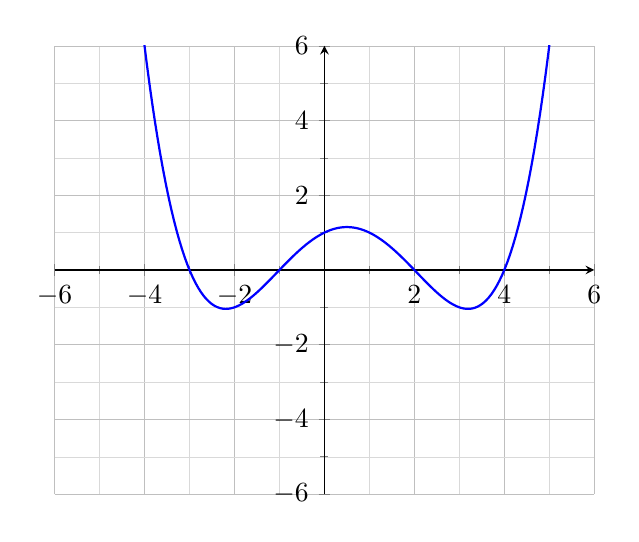
\begin{tikzpicture}
\begin{axis}%
    [grid=both,
     minor tick num=1,
     ymin=-6, ymax=6,
     xmin=-6, xmax=6,
     grid style={line width=.1pt, draw=gray!30},
     major grid style={line width=.2pt,draw=gray!50},
     axis lines=middle,
     enlargelimits=false,
     domain=-6:6,
     samples=200
    ]
    \addplot+[blue,mark=none,thick] {1/24*(x+3)*(x+1)*(x-2)*(x-4)};
  \end{axis}
\end{tikzpicture}
\end{center}
\end{exercise}
\begin{solution}[2in]

\end{solution}

\ifprintanswers\else\newpage\fi

\subsection{Finding the equation from key information}

\begin{exercise}
Write a polynomial, $p(x)$, in factored form given the following requirements:
\begin{itemize}
    \item degree 4;
    \item leading coefficient of 1;
    \item has zeros at $(1,0)$, $(-4,0)$, and $(2,0)$;
    \item $y$-intercept is $(0,-24)$.
\end{itemize}
\end{exercise}
\begin{solution}[3in]

\end{solution}

\begin{exercise}
Write a polynomial, $p(x)$, in factored form given the following requirements:
\begin{itemize}
    \item degree 3;
    \item leading coefficient of 1;
    \item has zeros at $(8,0)$, $(-4,0)$, and $(1,0)$;
    \item $y$-intercept is $(0,32)$.
\end{itemize}
\end{exercise}
\begin{solution}[2in]

\end{solution}

\begin{exercise}
Which of the following is the equation of a polynomial of degree 4 with zeros at
$(4,0)$ \& $(3,0)$ and $y$-intercept of $(0,96)$.
\end{exercise}
\begin{checkboxes}
\choice $y=(x+4)(x+3)(x+8)(x+1)$
\choice $y=(x+4)(x-3)(x-2)(x-1)$
\choice $y=(x-4)(x-3)(x+8)(x-1)$
\CorrectChoice $y=(x-4)(x-3)(x+2)(x+4)$
\end{checkboxes}
\begin{solution}[2in]

\end{solution}

\section{Division of Polynomials \& the Remainder Theorem}

\subsection{Long Division}

First I want to recall how we long divide numbers

\begin{exercise}
Use long division to find $24\div2$.
\end{exercise}
\begin{solution}[2in]

\end{solution}

We are now going to do the exact same thing with polynomials

\ifprintanswers\else\newpage\fi

\begin{exercise}
Divide $x^2+14x+45$ by $x+9$.
\end{exercise}
\begin{solution}[3in]

\end{solution}

\begin{exercise}
Divide $24x^3+2x^2-20x-6$ by $4x+3$.
\end{exercise}
\begin{solution}[3in]

\end{solution}

\begin{exercise}
Divide $25$ by $2$.
\end{exercise}
\begin{solution}[2in]

\end{solution}

\begin{exercise}
Divide $40x^2+31x-33$ by $5x+7$.
\end{exercise}
\begin{solution}[4in]

\end{solution}

\vspace{0.5em}

\begin{exercise}
Divide $-60x^3-40x^2+54x+38$ by $6x+4$.
\end{exercise}
\begin{solution}[4in]

\end{solution}

\begin{exercise}
Divide $6x^3-8x+4$ by $2x+6$.
\end{exercise}
\begin{solution}[4in]

\end{solution}

\begin{exercise}
The volume of a hexagonal prism is $12x^5+8x^4+9x^3-42x^2-33x-44$
and the area of the base is $2x^2+3x+4$. Find the height of the
prism.
\end{exercise}
\begin{solution}[4in]

\end{solution}

\subsection{Synthetic division}

This is a way to divide polynomial when the divisor is of the form
$\blank{x-c}{x-c}$

\begin{exercise}
Synthetically divide $x^2+14x+45$ by $x+9$
\end{exercise}
\begin{solution}[2.5in]

\end{solution}

\begin{exercise}
Use synthetic division to find $(x^4-10x^2-13x-50)\div(x+5)$
\end{exercise}
\begin{solution}[2.5in]

\end{solution}

\begin{exercise}
Synthetically divide $x^4-2x^2-4x-48$ by $x-3$
\end{exercise}
\begin{solution}[2.5in]

\end{solution}

\subsection{The Remainder Theorem}

\begin{theorem}[Remainder Theorem]\label{thm: remainder thm}
If a polynomial $f(x)$ is divided by $x-c$,
then remainder is $\blank{f(c)}{f(c)}$.
\end{theorem}

\begin{exercise}
What is the remainder of $g(x)=3x^3-20x^2+29x+30$ divided
by $x+2$
\end{exercise}
\begin{solution}[2in]

\end{solution}

\subsection{The Factor Theorem}

\begin{theorem}[Factor Theorem]\label{thm: factor thm}
$x-c$ is a factor of $f(x)$ if and only if
the remainder of $f(x)$ when divided by $x-c$ is $\blank{0}{0}$.

\vspace{0.5em}

Another way we can say this is $x-c$ is a factor of $f(x)$
if and only if $\blank{f(c)=0}{f(c)=0}$.
\end{theorem}

\begin{exercise}
Consider $f(x)=x^3-4x^2-47x+210$. When $f(x)$ is divided by $x+7$,
the remainder is $0$. What other binomials have a reminder of zero?
\end{exercise}
\begin{solution}[3.5in]

\end{solution}

\vspace{0.5em}

\begin{exercise}
For what values of $x$ is $x^3-12x^2+39x-28=0$?
\end{exercise}
\begin{solution}[4in]

\end{solution}

\section{Zeros of Polynomials}

First we need a rule for guessing zeros.

\subsection{Rational zero theorem}

\begin{theorem}[Rational Zero Theorem]\label{thm: rational zero thm}
If $f(x)=a_nx^n+a_{n-1}x^{n-1}+\cdots+a_1x+a_0$ has integer
coefficients, then every rational zero (fraction zero) of $f(x)$
is of the form $\dl\frac{p}{q}$, where $p$ is a factor
$\blank{a_0 (\text{the constant})}{a_0 (\text{the constant})}$ and
$q$ is a factor of $\blank{a_n (\text{the leading coefficient})}{a_n (\text{the leading coefficient})}$
\end{theorem}

\begin{exercise}
What are the possible rational zeros of $4x^5+12x^4-x-3$
\end{exercise}
\begin{solution}[1.5in]

\end{solution}

\begin{exercise}
What are the possible rational zeros of $x^3+2x^2-5x-6$
\end{exercise}
\begin{solution}[1in]

\end{solution}

\begin{exercise}
Find the rational zeros of $f(x)=x^3-5x^2-33x-27$.
\end{exercise}
\begin{solution}[3in]

\end{solution}

\subsection{Polynomials with complex zeros}

\begin{exercise}
Find all of the zeros of $f(x)=x^3+13x^2+57x+85$.
\end{exercise}
\begin{solution}[2in]

\end{solution}

\ifprintanswers\else\newpage\fi

\subsection{Linear Factorization Theorem}

\begin{theorem}[Linear Factorization Theorem]
Any polynomial $f(x)$ can be written as
\[
f(x)=\blank{a_n(x-c_1)(x-c_2)\cdots(x-c_n)}{a_n(x-c_1)(x-c_2)\cdots(x-c_n)}
\]
where $a_n$ is the leading coefficient, the degree of $f(x)$ is $n$,
and $c_1,c_2,\ldots,c_n$ are the complex zeros of $f(x)$ (not necessarily distinct).
\end{theorem}

\begin{exercise}
Find a third degree polynomial that has an output of $16$ when $x=2$
and zeros of $1$ and $-2i$.
\end{exercise}
\begin{solution}[4in]

\end{solution}

\ifprintanswers\else\newpage\fi

\begin{exercise}
Find a third degree polynomial that has an output of $20$ when $x=0$
and zeros of $4$ and $-1+3i$.
\end{exercise}
\begin{solution}[6in]

\end{solution}

\subsection{Descartes' Rule of Signs}

The following is occasionally useful when guessing zeros for the rational zero theorem.

\begin{prop}
\text{}
\begin{enumerate}[1)]
    \item The number of positive real zeros of a polynomial $f(x)$
    is either the number of sign changes of $\blank{f(x)}{f(x)}$
    or less a positive even integer.
    \item The number of negative real zeros of a polynomial $f(x)$
    is either the number of sign changes of $\blank{f(-x)}{f(-x)}$
    or less a positive even integer.
\end{enumerate}
\end{prop}

\vspace{1em}

\begin{exercise}
For $f(x)=7x^4+2x^3+4x^2-6x+5$, what are the possible combinations of positive, negative, and imaginary zeros of $f(x)$.
\end{exercise}
\begin{solution}[2.5in]

\end{solution}

\begin{exercise}
For $f(x)=x^4-2x^3+4x^2-3x+17$, what are the possible combinations of positive, negative, and imaginary zeros of $f(x)$.
\end{exercise}
\begin{solution}[2.5in]

\end{solution}

\begin{exercise}
For $f(x)=x^6-2x^5+7x^4+5x^3-7x^2+3x-10$, what are the possible combinations of positive, negative, and imaginary zeros of $f(x)$.
\end{exercise}
\begin{solution}[2.5in]

\end{solution}


\section{Rational Functions}

\begin{align*}
\text{rational numbers}&\longleftrightarrow\text{fractions of integers}\\
\text{rational functions}&\longleftrightarrow\blank{\text{fractions of polynomials}}{\text{fraction of polynomials}}
\end{align*}

\begin{definition}\label{def: rational functions}
A function $f(x)$ is a \emph{rational function} if
\[
f(x)=
\]
where $p(x)$ and $q(x)$ are \blank{polynomials}{polynomials}
\end{definition}

\begin{example}
\text{}
\begin{itemize}
    \item $\dl\blank{f(x)=\frac{3x+2}{5x^2-7x+1}}{f(x)=\frac{3x+2}{5x^2-7x+1}}$
    \item $\dl\blank{f(x)=\frac{x^7+x-3}{x^2+2x+3}}{f(x)=\frac{x^7+x-3}{x^2+2x+3}}$
\end{itemize}
\end{example}

\begin{nonex}
\text{}
\begin{itemize}
\item $\blank{g(x)=\frac{3x+2}{\sqrt{3x+7}}}{g(x)=\frac{3x+2}{\sqrt{3x+7}}}$
\end{itemize}
\end{nonex}

\begin{note}
Here is some useful notation that we will see when working with rational functions:
\begin{itemize}
    \item $\blank{x\rightarrow a^+}{x\rightarrow a^+}$ - $x$ approaches $a$ from the right/above.
    \item $\blank{x\rightarrow a^-}{x\rightarrow a^-}$ - $x$ approaches $a$ from the left/below.
    \item $\blank{x\rightarrow\infty}{x\rightarrow\infty}$ - $x$ approaches infinity.
    \item $\blank{x\rightarrow-\infty}{x\rightarrow-\infty}$ - $x$ approaches negative infinity.
\end{itemize}
\end{note}

\begin{definition}
A \emph{vertical asymptote} (VA) is a vertical line
$x=a$ such that $f(x)\rightarrow\blank{\pm\infty}{\pm\infty}$ as
$x\rightarrow\blank{a^{\pm}}{a^{\pm}}$
\end{definition}

\ifprintanswers
\else
\begin{center}

\begin{tikzpicture}[scale=0.4]
\draw[step=1cm,gray,very thin] (-5,-5) grid (5,5);
\draw (-5,0) -- (5,0);
\draw (0,-5) -- (0,5);
\end{tikzpicture}
\hspace{0.25in}

\begin{tikzpicture}[scale=0.4]
\draw[step=1cm,gray,very thin] (-5,-5) grid (5,5);
\draw (-5,0) -- (5,0);
\draw (0,-5) -- (0,5);
\end{tikzpicture}
\hspace{0.25in}

\begin{tikzpicture}[scale=0.4]
\draw[step=1cm,gray,very thin] (-5,-5) grid (5,5);
\draw (-5,0) -- (5,0);
\draw (0,-5) -- (0,5);
\end{tikzpicture}
\end{center}
\fi

\ifprintanswers\else\newpage\fi

\begin{definition}
A \emph{horizontal asymptote} (HA) is a horizontal line
$y=b$ such that $f(x)\rightarrow\blank{b^{\pm}}{b^{\pm}}$ as
$x\rightarrow\blank{\pm\infty}{\pm\infty}$
\end{definition}

\ifprintanswers
\else
\begin{center}

\begin{tikzpicture}[scale=0.4]
\draw[step=1cm,gray,very thin] (-5,-5) grid (5,5);
\draw (-5,0) -- (5,0);
\draw (0,-5) -- (0,5);
\end{tikzpicture}
\hspace{0.25in}

\begin{tikzpicture}[scale=0.4]
\draw[step=1cm,gray,very thin] (-5,-5) grid (5,5);
\draw (-5,0) -- (5,0);
\draw (0,-5) -- (0,5);
\end{tikzpicture}
\hspace{0.25in}

\begin{tikzpicture}[scale=0.4]
\draw[step=1cm,gray,very thin] (-5,-5) grid (5,5);
\draw (-5,0) -- (5,0);
\draw (0,-5) -- (0,5);
\end{tikzpicture}
\end{center}
\fi

\subsection{Describe the behavior of rational functions using their graph}

\begin{exercise}
Describe the behavior of $f(x)$ below:
\begin{center}
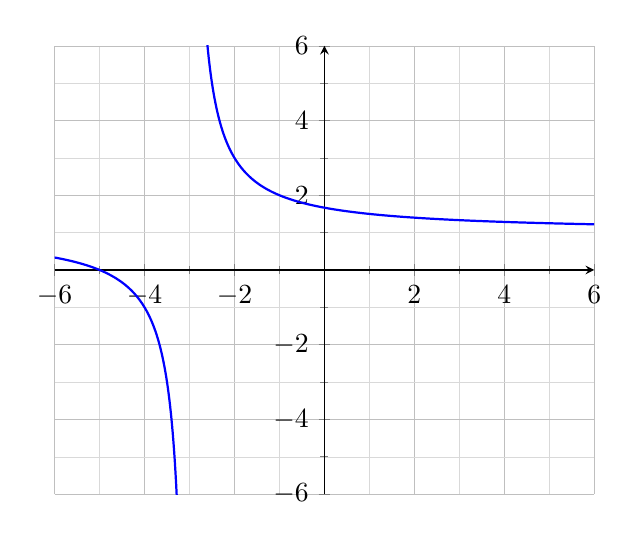
\begin{tikzpicture}
\begin{axis}%
    [grid=both,
     minor tick num=1,
     ymin=-6, ymax=6,
     xmin=-6, xmax=6,
     grid style={line width=.1pt, draw=gray!30},
     major grid style={line width=.2pt,draw=gray!50},
     axis lines=middle,
     enlargelimits=false,
    ]
    \addplot+[blue,mark=none,thick,samples=800,restrict y to domain=-10:10,domain=-6:6] {(x+5)/(x+3)};
\end{axis}
\end{tikzpicture}
\end{center}
\end{exercise}
\begin{solution}[2in]

\end{solution}

\ifprintanswers\else\newpage\fi

\begin{exercise}
Describe the behavior of $f(x)$ below:
\begin{center}
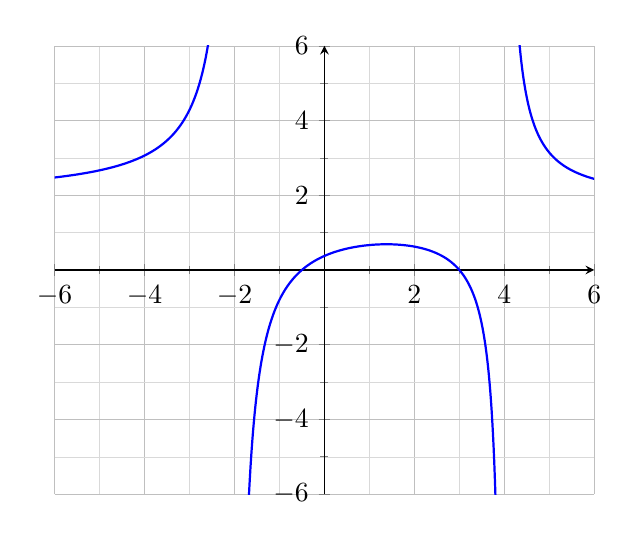
\begin{tikzpicture}
\begin{axis}%
    [grid=both,
     minor tick num=1,
     ymin=-6, ymax=6,
     xmin=-6, xmax=6,
     grid style={line width=.1pt, draw=gray!30},
     major grid style={line width=.2pt,draw=gray!50},
     axis lines=middle,
     enlargelimits=false,
    ]
    \addplot+[blue,mark=none,thick,samples=800,restrict y to domain=-10:10,domain=-6:6] {((2*x+1)*(x-3))/((x+2)*(x-4))};
\end{axis}
\end{tikzpicture}
\end{center}
\end{exercise}
\begin{solution}[2in]

\end{solution}

\subsection{Finding vertical asymptotes}

\begin{fact}
The function $\dl f(x)=\frac{p(x)}{q(x)}$ has a VA at $x=a$
if \blank{$p(a)\neq0$ and $q(a)=0$}{$p(a)\neq0$ and $q(a)=0$}.

\vspace{1em}

If both \blank{$p(a)=0$ and $q(a)=0$}{$p(a)=0$ and $q(a)=0$}, then
either $a$ is a \blank{removable discontinuity/singularity}{removable discontinuity/singularity} if we can simplify $f(x)$ such
that $a$ no longer makes the denominator \blank{$0$}{$0$}.

\vspace{1em}

If the denominator is still \blank{$0$}{$0$}, but the numerator is not, then it is a VA and is called an \blank{essential singularity}{essential singularity}.
\end{fact}

\ifprintanswers\else\newpage\fi

\begin{exercise}
Consider
\[
f(x)=\frac{x^3-x^2-2x}{x^2+x}.
\]
Does $f(x)$ have any removable discontinuities?
\end{exercise}
\begin{solution}[3.5in]

\end{solution}

\begin{exercise}
Consider
\[
f(x)=\frac{x^2-36}{x^3-2x^2-24x}.
\]
What are the vertical asymptotes of $f(x)$ (if any)?
\end{exercise}
\begin{solution}[3.5in]

\end{solution}

\subsection{Finding horizontal asymptotes}

\begin{fact}
Let $\dl f(x)=\frac{a_nx^n+\cdots+a_1x+a_0}{b_mx^m+\cdots+b_1x+b_0}$.
To find the horizontal asymptote we need to compare the degrees $m$ and $n$:
\begin{itemize}
\item \blank{$n>m$}{$n>m$} $\Rightarrow$ there is no HA.
\item \blank{$n<m$}{$n<m$} $\Rightarrow$ the $x$-axis $(y=0)$
is the HA.
\item \blank{$n=m$}{$n=m$} $\Rightarrow$ $\dl y=\frac{a_n}{b_m}$
is the HA.
\end{itemize}
\end{fact}

\begin{exercise}
What is the HA (if one) of
\[
f(x)=\frac{9x}{3x+1}
\]
\end{exercise}
\begin{solution}[1in]

\end{solution}

\begin{exercise}
What is the HA (if one) of
\[
g(x)=\frac{7x^5+4}{3x^6+x+3}
\]
\end{exercise}
\begin{solution}[1in]

\end{solution}

\begin{exercise}
What is the HA (if one) of
\[
h(x)=\frac{x^2+1}{x+1}
\]
\end{exercise}
\begin{solution}[1in]

\end{solution}

\ifprintanswers\else\newpage\fi

As we saw, some rational functions do not have a HA, but some have the following instead

\begin{definition}\label{def: SA}
If $\dl f(x)=\frac{p(x)}{q(x)}$ is a rational function and
$\deg(p(x))=\deg(q(x))+1$, then $f(x)$ has a \emph{slant asymptote} (SA)
which is a line $y=mx+b$ that $f(x)$ approaches as $x\rightarrow\blank{\pm\infty}{\pm\infty}$
\end{definition}

\begin{ques}
How do you find a SA?
\end{ques}

We use division! Since the denominator's degree is one less than the numerator's degree the quotient will have to have degree 1.

\begin{exercise}
If
\[
h(x)=\frac{x^2+1}{x+1}
\]
what is its SA?
\end{exercise}
\begin{solution}[2in]

\end{solution}

\subsection{Graphing rational functions}

Here is the general strategy if $\dl f(x)=\frac{p(x)}{q(x)}$
is fully simplified.

\begin{enumerate}[1)]
    \item Find the $y$-intercept (if there is one) by finding $\blank{f(0)}{f(0)}$.
    \item Find $x$-intercept (if any) by solving $\blank{p(x)=0}{p(x)=0}$.
    \item Find VA by solving $\blank{q(x)=0}{q(x)=0}$.
    \item Find HA (if there is one) by comparing degrees.
    \begin{enumerate}[4.5)]
        \item Find the SA (if there is one) using division.
    \end{enumerate}
    \item Plot extra points between the intercepts and VA as needed.
\end{enumerate}

\ifprintanswers\else\newpage\fi

\begin{exercise}
Graph $\dl f(x)=\frac{x-1}{x-4}$
\end{exercise}
\ifprintanswers
\else
\begin{center}

\begin{tikzpicture}[scale=0.5]
\draw[step=1cm,gray,very thin] (-8,-8) grid (8,8);
\draw (-8,0) -- (8,0);
\draw (0,-8) -- (0,8);
\end{tikzpicture}
\end{center}
\fi
\begin{solution}[2in]

\end{solution}

\ifprintanswers\else\newpage\fi

\begin{exercise}
Graph $\dl f(x)=\frac{(x-2)(x-5)}{(x-3)^2}$
\end{exercise}
\ifprintanswers
\else
\begin{center}

\begin{tikzpicture}[scale=0.5]
\draw[step=1cm,gray,very thin] (-8,-8) grid (8,8);
\draw (-8,0) -- (8,0);
\draw (0,-8) -- (0,8);
\end{tikzpicture}
\end{center}
\fi
\begin{solution}[4in]

\end{solution}

\ifprintanswers\else\newpage\fi

\subsection{Identifying rational functions from their graphs}

\begin{exercise}
Identify the rational function graphed below. Note the $x$-intercept of $x=-3$ and $(-1,-2)$ is a point on the graph.
\begin{center}
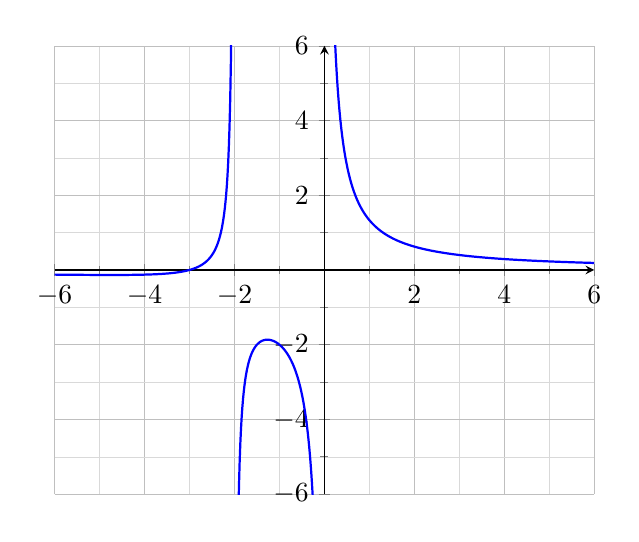
\begin{tikzpicture}
\begin{axis}%
    [grid=both,
     minor tick num=1,
     ymin=-6, ymax=6,
     xmin=-6, xmax=6,
     grid style={line width=.1pt, draw=gray!30},
     major grid style={line width=.2pt,draw=gray!50},
     axis lines=middle,
     enlargelimits=false,
    ]
    \addplot+[blue,mark=none,thick,samples=800,restrict y to domain=-10:10,domain=-6:6] {(x+3)/(x*(x+2))};
\end{axis}
\end{tikzpicture}
\end{center}
\end{exercise}
\begin{solution}[2in]

\end{solution}

\ifprintanswers\else\newpage\fi

\begin{exercise}
Identify the rational function graphed below. Note the $x$-intercept of $x=3$ and $y$-intercept at $-3$.
\begin{center}
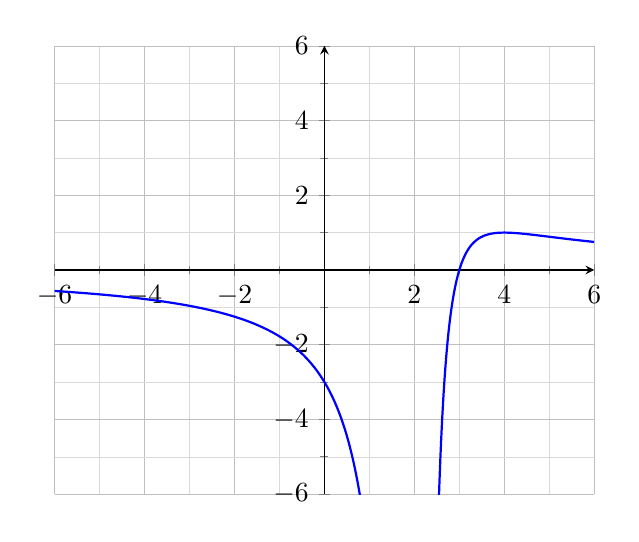
\begin{tikzpicture}
\begin{axis}%
    [grid=both,
     minor tick num=1,
     ymin=-6, ymax=6,
     xmin=-6, xmax=6,
     grid style={line width=.1pt, draw=gray!30},
     major grid style={line width=.2pt,draw=gray!50},
     axis lines=middle,
     enlargelimits=false,
    ]
    \addplot+[blue,mark=none,thick,samples=800,restrict y to domain=-10:10,domain=-6:6] {4*(x-3)/((x-2)^2)};
\end{axis}
\end{tikzpicture}
\end{center}
\end{exercise}
\begin{solution}[2in]

\end{solution}

\newpage

\section{Polynomial and Rational Inequalities}

Just as linear inequalities start with solving the "equation", the same is true of
polynomial and rational inequalities.

\subsection{Polynomial inequalities}

Here is the procedure for solving inequalties such as $f(x)>0,~f(x)<0,~f(x)\geq0,~f(x)\leq0$ where
$f(x)$ is a polynomial:
\begin{enumerate}
    \item Set one side to $\blank{0}{0}$
    \item Solve $\blank{f(x)=0}{f(x)=0}$
    \item Plot those solutions on a \blank{number line}{number line}
    \item Find test values in between these numbers and test to find the \blank{sign}{sign}
    \item Choose correct interval(s) based on original inequality $\blank{>0,\geq0\longleftrightarrow+}{>0,\geq0\longleftrightarrow+}$ and
    $\blank{<0,\leq0\longleftrightarrow-}{<0,\leq0\longleftrightarrow-}$
\end{enumerate}
\vspace{0.5em}

\begin{exercise}
Solve $x^2-x>20$ for $x$. (Give your answer in interval notation)
\end{exercise}
\begin{solution}[3in]

\end{solution}

\ifprintanswers\else\newpage\fi

\begin{exercise}
Solve $2x^2\leq-6x-4$ for $x$. (Give your answer in interval notation)
\end{exercise}
\begin{solution}[4in]

\end{solution}

\vspace{0.5em}

\begin{exercise}
Solve $x^3+3x^2\leq x+3$ for $x$. (Give your answer in interval notation)
\end{exercise}
\begin{solution}[4in]

\end{solution}

\subsubsection*{Position of a free-falling object near earth's surface}

\begin{fact}
The position of a free falling object (in feet) at time $t$ can be described by the following quadratic:
\[
s(t)=\blank{-16t^2+v_0t+s_0}{-16t^2+v_0t+s_0}
\]
where $\blank{v_0}{v_0}$ is the initial velocity and $\blank{s_0}{s_0}$ is the initial position.
\end{fact}

\vspace{0.5em}

\begin{exercise}
Given the following position function, find the interval of time that the object is more than $64$
feet above the ground.
\[
s(t)=-16t^2+80t
\]
\end{exercise}
\begin{solution}[3in]

\end{solution}

\subsection{Rational inequalities}

What follows is the procedure for solving rational inequalities.
\begin{enumerate}
    \item Write the inequality with $0$ on one side
    \item Combine the fractions on the other side as \blank{a single fraction}{a single fraction}
    \item Set the numerator and denominator equal to $\blank{0}{0}$
    \item Plot on number line
    \item Test values
    \item Choose correct interval(s)
\end{enumerate}

\vspace{0.5em}

\begin{exercise}
Solve the following for $x$:
\[
\frac{2x}{x+1}\geq1
\]
\end{exercise}
\begin{solution}[3.5in]

\end{solution}

\begin{exercise}
Solve the following for $x$:
\[
\frac{x-2}{x+2}\leq2
\]
\end{exercise}
\begin{solution}[3.5in]

\end{solution}

\begin{exercise}
Find the solution to the following inequality in interval notation:
\[
\frac{2}{x+3}\leq\frac{1}{x-3}
\]
\end{exercise}
\begin{solution}[3.5in]

\end{solution}

\begin{exercise}
Find the solution to the following inequality in interval notation:
\[
\frac{3}{x+7}\geq\frac{2}{x-5}
\]
\end{exercise}
\begin{solution}[3.5in]

\end{solution}
